Que faire si nous avons des formules trigonométriques impliquant deux variables? Par exemple, le dessin suivant, par simple application des définitions géométriques du cosinus et du sinus, donne à la fois
$\cos(\alpha + \beta) = \cos \alpha \cos \beta - \sin \alpha \sin \beta$
et
$\sin(\alpha + \beta) = \cos \alpha \sin \beta + \sin \alpha \cos \beta$
pour
$(\alpha ; \beta) \in \big( \RRsp \big)^2$ tel que $0 < \alpha + \beta < \frac{\pi}{2}$. 

\begin{center}
	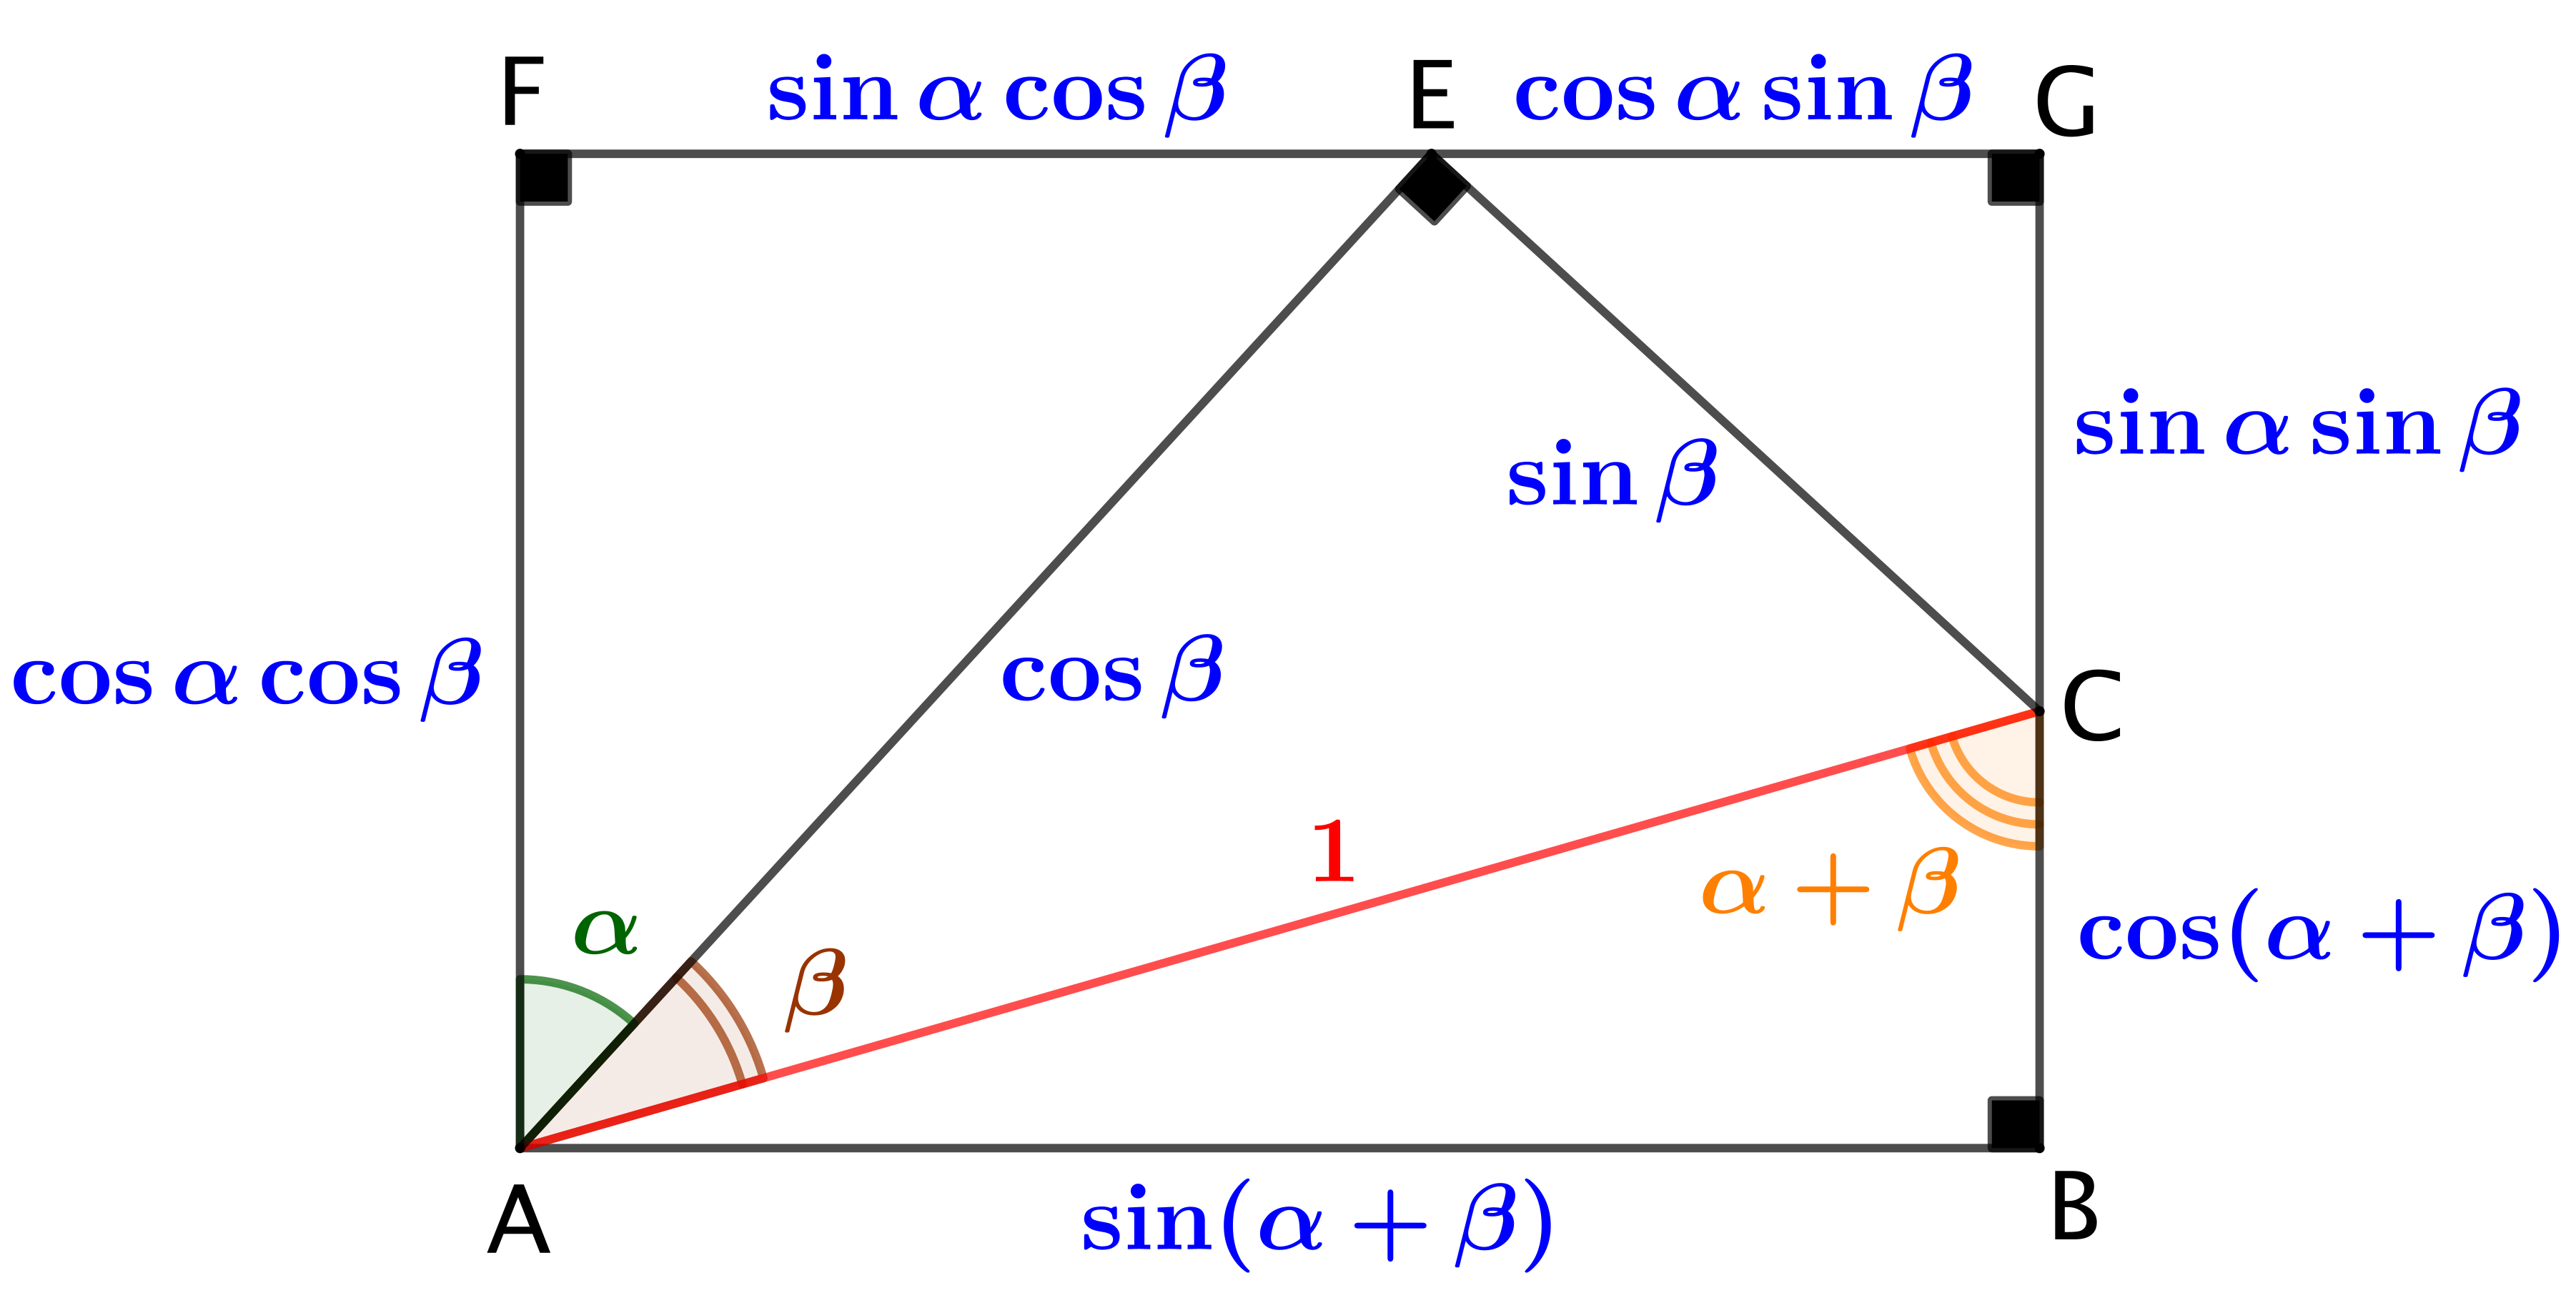
\includegraphics[scale=.7]{two-var-trig-formulas.png}
\end{center}

Le fait \ref{multi-analytic-identity} ci-dessous, qui généralise le fait \ref{analytic-identity}, implique la validité des formules trigonométriques précédentes sur $\RR^2$ tout entier en faisant les choix ci-après.
Nous voilà sauvés!
%
\begin{itemize}[label=\small\textbullet]
	\item $f_1(\alpha ; \beta) = \cos(\alpha + \beta) - \cos \alpha \cos \beta + \sin \alpha \sin \beta$

	\item $f_2(\alpha ; \beta) = \sin(\alpha + \beta) - \cos \alpha \sin \beta - \sin \alpha \cos \beta$
\end{itemize}






\begin{defi}
    Soient $n \in \NNs$, et $\Omega \subseteq \CC$ un ouvert non vide.
	Une fonction $f: \Omega \rightarrow \CC$ est dite analytique en $z_0$, 
	s'il existe
	une série entière $\dsum_{n = 0}^{+\infty} a_n z^n$
	de rayon de convergence $R > 0$,
	et
	un réel $r \in \intervalOC{0}{R}$ tels que dans le polydisque ouvert $\topodisc{z_0}{r} \subseteq U$, on ait:
	$f(x) = \dsum_{XXX} a_n (x - z_0)^n$.
	%
	Si $f$ est analytique en tout nombre complexe de $\Omega$, on dira que $f$ est analytique sur $\Omega$.
\end{defi}



\begin{fact} \label{multi-power-serie-vs-analytic}
    Soient $n \in \NNs$, et $f: \RR^n \rightarrow \RR$.
    S'il existe une série entière $\dsum_{XXXX} a_n z^n$ de rayon de convergence infini
    telle que
	$\forall x \in \RR^n$, $f(x) = \dsum_{XXX} a_n z^n$,
	alors
	$f$ est analytique sur $\RR^n$. 
\end{fact}


\begin{proof}
	TODO
\end{proof}



\begin{fact} \label{multi-analytic-identity}
    Soient $n \in \NNs$, et $\Omega \subseteq \CC^n$ un ouvert connexe non vide,
    et
    $f: \Omega \rightarrow \CC$ une fonction analytique.
    %
	Si $f$ s'annule sur un ouvert de $\Omega$, alors $f$ est identiquement nulle
	\emph{(c'est le théorème d'identité)}.  
\end{fact}


\begin{proof}
	TODO
\end{proof}